\documentclass{standalone}
\usepackage{pgfplots}
\usepackage{amsmath}
\usetikzlibrary{calc}
\usetikzlibrary{decorations.markings}

\pgfplotsset{compat=newest}

\tikzset{decorated arrowsb/.style={
		postaction={
			decorate,
			decoration={
				markings,
				mark=between positions 0.49 and 0.51 step 15mm with {\arrow[black]{stealth}}}
		}
}}
\tikzset{decorated arrowsr/.style={
		postaction={
			decorate,
			decoration={
				markings,
				mark=between positions 0.49 and 0.51 step 15mm with {\arrow[red]{stealth}}}
		}
}}
\tikzset{decorated arrowsbl/.style={
		postaction={
			decorate,
			decoration={
				markings,
				mark=between positions 0.49 and 0.51 step 15mm with {\arrow[blue]{stealth}}}
		}
}}

\begin{document}
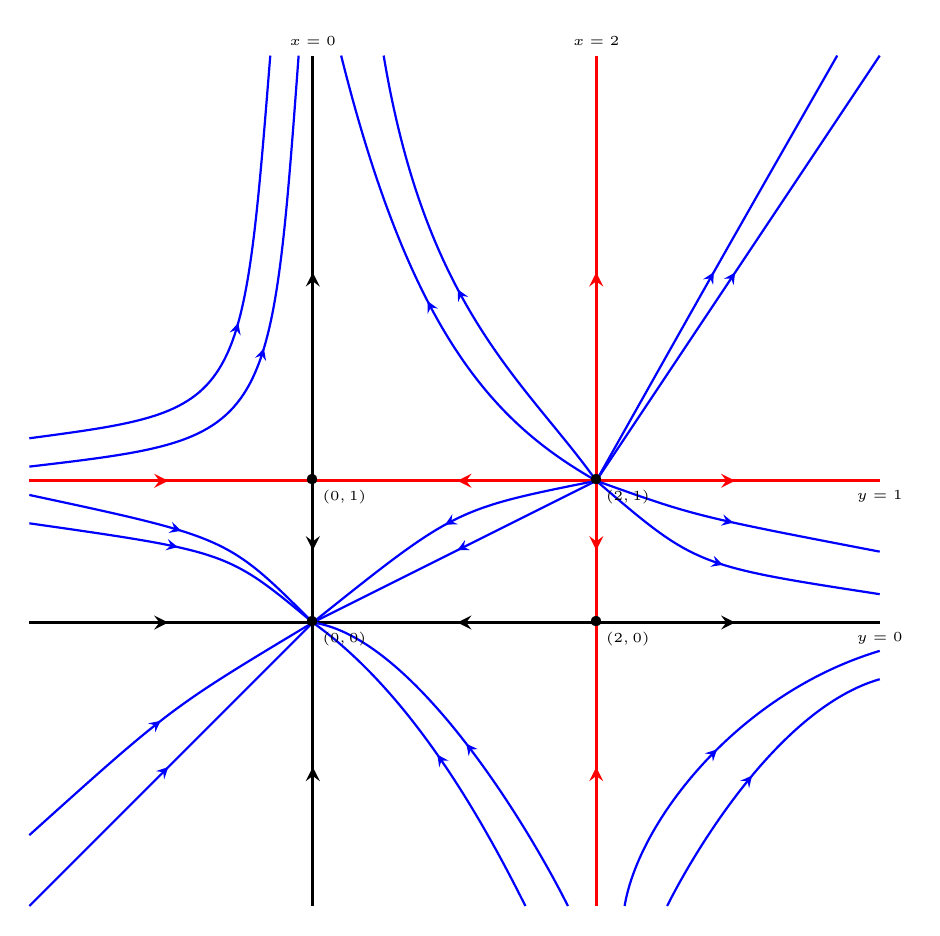
\begin{tikzpicture}[scale=1.8]
  \draw (0,-2)-- (0,4) node[above]{\tiny{$x=0$}};
  \draw (-2, 0)--(4,0) node[below]{\tiny{$y=0$}};
  \draw (2,-2)-- (2,4) node[above]{\tiny{$x=2$}};
  \draw (-2, 1)--(4,1) node[below]{\tiny{$y=1$}};
  \draw[very thick, color=black, decorated arrowsb] (-2, 0)--(0,0);
  \draw[very thick, color=black, decorated arrowsb] (2, 0)--(0,0);
  \draw[very thick, color=black, decorated arrowsb] (0,1)--(0,4);
  \draw[very thick, color=black, decorated arrowsb] (0,-2)--(0,0);
  \draw[very thick, color=black, decorated arrowsb] (2, 0)--(4,0);
  \draw[very thick, color=black, decorated arrowsb] (0,1)--(0,0);

  \draw[very thick, color=red, decorated arrowsr] (-2, 1)--(0,1);
  \draw[very thick, color=red, decorated arrowsr] (2, 1)--(0,1);
  \draw[very thick, color=red, decorated arrowsr] (2,1)--(2,4);
  \draw[very thick, color=red, decorated arrowsr] (2,-2)--(2,0);
  \draw[very thick, color=red, decorated arrowsr] (2, 1)--(4,1);
  \draw[very thick, color=red, decorated arrowsr] (2,1)--(2,0);

  \draw[thick, color=blue, decorated arrowsbl] (-2, 1.1).. controls (-0.3,1.3)..(-0.1, 4);
  \draw[thick, color=blue, decorated arrowsbl] (-2, 1.3).. controls (-0.5,1.5)..(-0.3, 4);
  \draw[thick, color=blue, decorated arrowsbl] (-2, 0.9).. controls (-0.6, 0.6)..(0, 0);
  \draw[thick, color=blue, decorated arrowsbl] (-2, 0.7).. controls (-0.6, 0.5)..(0, 0);
  \draw[thick, color=blue, decorated arrowsbl] (-2, -2)--(0, 0);
  \draw[thick, color=blue, decorated arrowsbl] (-2, -1.5).. controls (-1, -0.6)..(0, 0);
  \draw[thick, color=blue, decorated arrowsbl] (2, 1).. controls (1.3, 1.4) and (0.7, 2)..(0.2, 4);
  \draw[thick, color=blue, decorated arrowsbl] (2, 1).. controls (1.5, 1.7) and (0.8, 2.2)..(0.5, 4);
  \draw[thick, color=blue, decorated arrowsbl] (2, 1)--(0, 0);
  \draw[thick, color=blue, decorated arrowsbl] (2, 1).. controls (1, 0.8)..(0, 0);
  \draw[thick, color=blue, decorated arrowsbl] (1.8, -2).. controls (1.5, -1.4) and (0.7, -0.1)..(0, 0);
  \draw[thick, color=blue, decorated arrowsbl] (1.5, -2).. controls (1.2, -1.4) and (0.7, -0.5)..(0, 0);
  \draw[thick, color=blue, decorated arrowsbl] (2.2, -2).. controls (2.3, -1.4) and (3, -0.5)..(4, -0.2);
  \draw[thick, color=blue, decorated arrowsbl] (2.5, -2).. controls (2.7, -1.6) and (3.3, -0.6)..(4, -0.4);
  \draw[thick, color=blue, decorated arrowsbl] (2, 1).. controls (2.7, 0.4)..(4, 0.2);
  \draw[thick, color=blue, decorated arrowsbl] (2, 1).. controls (2.7, 0.75)..(4, 0.5);
  \draw[thick, color=blue, decorated arrowsbl] (2, 1)--(4, 4);
  \draw[thick, color=blue, decorated arrowsbl] (2, 1)..controls (2.9, 2.6)..(3.7, 4);

  \node at (0,0) {\textbullet};
  \node[below right] at (0,0){\tiny{$(0,0)$}};
  \node at (2,0) {\textbullet};
  \node[below right] at (2,0){\tiny{$(2,0)$}};
  \node at (0,1) {\textbullet};
  \node[below right] at (0,1){\tiny{$(0,1)$}};
  \node at (2,1) {\textbullet};
  \node[below right] at (2,1){\tiny{$(2,1)$}};
\end{tikzpicture}
\end{document}